% Created by tikzDevice version 0.11 on 2018-04-09 15:27:55
% !TEX encoding = UTF-8 Unicode
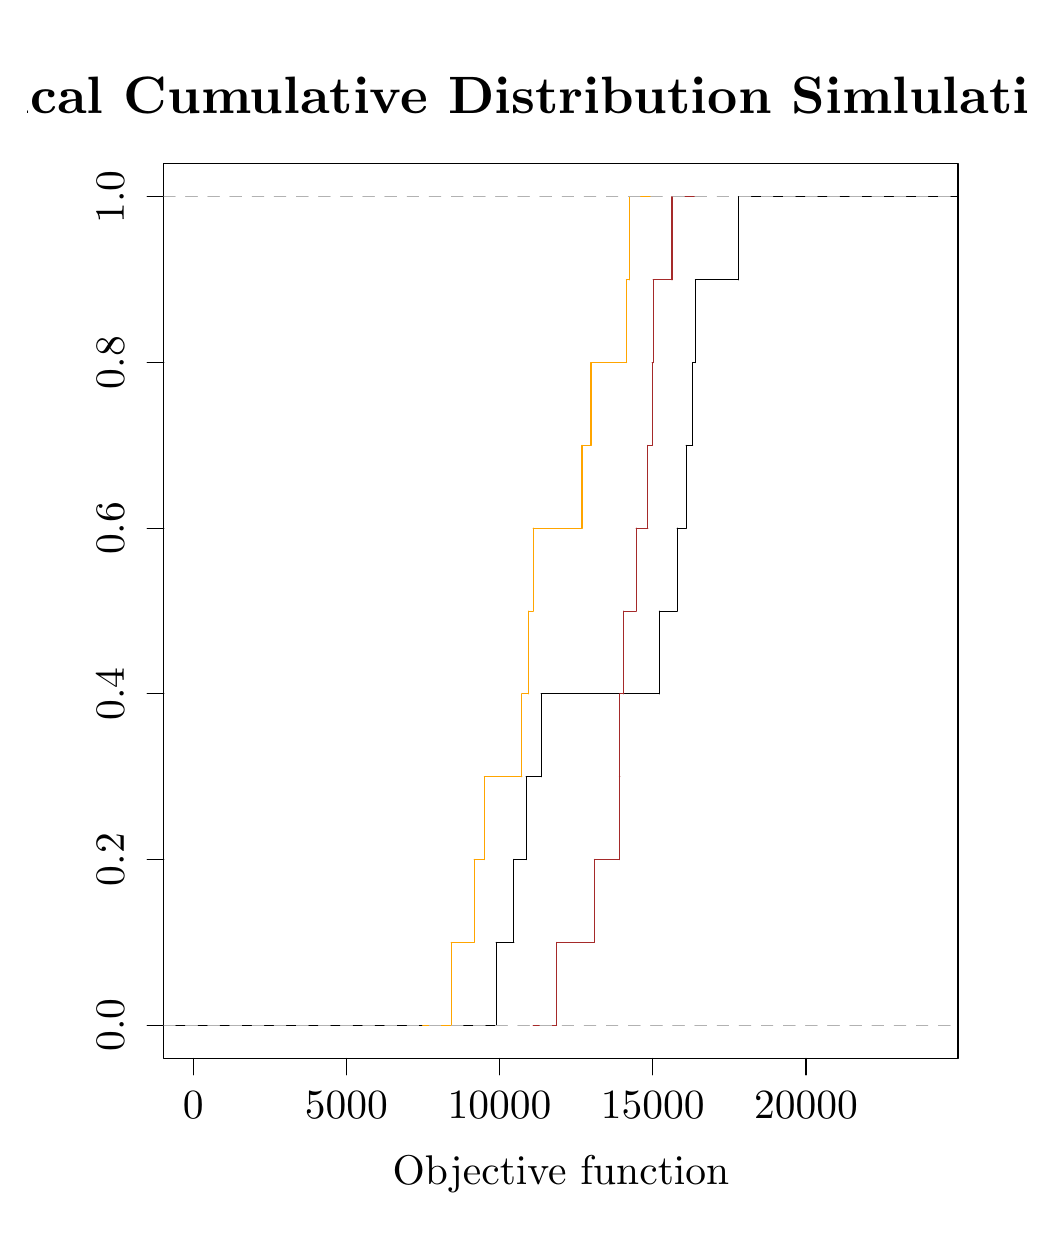
\begin{tikzpicture}[x=1pt,y=1pt]
\definecolor{fillColor}{RGB}{255,255,255}
\path[use as bounding box,fill=fillColor,fill opacity=0.00] (0,0) rectangle (361.35,433.62);
\begin{scope}
\path[clip] (  0.00,  0.00) rectangle (361.35,433.62);
\definecolor{drawColor}{RGB}{0,0,0}

\path[draw=drawColor,line width= 0.4pt,line join=round,line cap=round] ( 59.83, 61.20) -- (281.24, 61.20);

\path[draw=drawColor,line width= 0.4pt,line join=round,line cap=round] ( 59.83, 61.20) -- ( 59.83, 55.20);

\path[draw=drawColor,line width= 0.4pt,line join=round,line cap=round] (115.18, 61.20) -- (115.18, 55.20);

\path[draw=drawColor,line width= 0.4pt,line join=round,line cap=round] (170.53, 61.20) -- (170.53, 55.20);

\path[draw=drawColor,line width= 0.4pt,line join=round,line cap=round] (225.89, 61.20) -- (225.89, 55.20);

\path[draw=drawColor,line width= 0.4pt,line join=round,line cap=round] (281.24, 61.20) -- (281.24, 55.20);

\node[text=drawColor,anchor=base,inner sep=0pt, outer sep=0pt, scale=  1.50] at ( 59.83, 39.60) {0};

\node[text=drawColor,anchor=base,inner sep=0pt, outer sep=0pt, scale=  1.50] at (115.18, 39.60) {5000};

\node[text=drawColor,anchor=base,inner sep=0pt, outer sep=0pt, scale=  1.50] at (170.53, 39.60) {10000};

\node[text=drawColor,anchor=base,inner sep=0pt, outer sep=0pt, scale=  1.50] at (225.89, 39.60) {15000};

\node[text=drawColor,anchor=base,inner sep=0pt, outer sep=0pt, scale=  1.50] at (281.24, 39.60) {20000};

\path[draw=drawColor,line width= 0.4pt,line join=round,line cap=round] ( 49.20, 73.17) -- ( 49.20,372.45);

\path[draw=drawColor,line width= 0.4pt,line join=round,line cap=round] ( 49.20, 73.17) -- ( 43.20, 73.17);

\path[draw=drawColor,line width= 0.4pt,line join=round,line cap=round] ( 49.20,133.03) -- ( 43.20,133.03);

\path[draw=drawColor,line width= 0.4pt,line join=round,line cap=round] ( 49.20,192.88) -- ( 43.20,192.88);

\path[draw=drawColor,line width= 0.4pt,line join=round,line cap=round] ( 49.20,252.74) -- ( 43.20,252.74);

\path[draw=drawColor,line width= 0.4pt,line join=round,line cap=round] ( 49.20,312.59) -- ( 43.20,312.59);

\path[draw=drawColor,line width= 0.4pt,line join=round,line cap=round] ( 49.20,372.45) -- ( 43.20,372.45);

\node[text=drawColor,rotate= 90.00,anchor=base,inner sep=0pt, outer sep=0pt, scale=  1.50] at ( 34.80, 73.17) {0.0};

\node[text=drawColor,rotate= 90.00,anchor=base,inner sep=0pt, outer sep=0pt, scale=  1.50] at ( 34.80,133.03) {0.2};

\node[text=drawColor,rotate= 90.00,anchor=base,inner sep=0pt, outer sep=0pt, scale=  1.50] at ( 34.80,192.88) {0.4};

\node[text=drawColor,rotate= 90.00,anchor=base,inner sep=0pt, outer sep=0pt, scale=  1.50] at ( 34.80,252.74) {0.6};

\node[text=drawColor,rotate= 90.00,anchor=base,inner sep=0pt, outer sep=0pt, scale=  1.50] at ( 34.80,312.59) {0.8};

\node[text=drawColor,rotate= 90.00,anchor=base,inner sep=0pt, outer sep=0pt, scale=  1.50] at ( 34.80,372.45) {1.0};

\path[draw=drawColor,line width= 0.4pt,line join=round,line cap=round] ( 49.20, 61.20) --
	(336.15, 61.20) --
	(336.15,384.42) --
	( 49.20,384.42) --
	( 49.20, 61.20);
\end{scope}
\begin{scope}
\path[clip] (  0.00,  0.00) rectangle (361.35,433.62);
\definecolor{drawColor}{RGB}{0,0,0}

\node[text=drawColor,anchor=base,inner sep=0pt, outer sep=0pt, scale=  1.90] at (192.68,402.46) {\bfseries Empirical Cumulative Distribution Simlulation values};

\node[text=drawColor,anchor=base,inner sep=0pt, outer sep=0pt, scale=  1.50] at (192.68, 15.60) {Objective function};
\end{scope}
\begin{scope}
\path[clip] ( 49.20, 61.20) rectangle (336.15,384.42);
\definecolor{drawColor}{RGB}{0,0,0}

\path[draw=drawColor,line width= 0.4pt,line join=round,line cap=round] (  0.00, 73.17) -- (169.29, 73.17);

\path[draw=drawColor,line width= 0.4pt,line join=round,line cap=round] (169.29,103.10) -- (175.65,103.10);

\path[draw=drawColor,line width= 0.4pt,line join=round,line cap=round] (175.65,133.03) -- (180.10,133.03);

\path[draw=drawColor,line width= 0.4pt,line join=round,line cap=round] (180.10,162.95) -- (185.51,162.95);

\path[draw=drawColor,line width= 0.4pt,line join=round,line cap=round] (185.51,192.88) -- (228.24,192.88);

\path[draw=drawColor,line width= 0.4pt,line join=round,line cap=round] (228.24,222.81) -- (234.67,222.81);

\path[draw=drawColor,line width= 0.4pt,line join=round,line cap=round] (234.67,252.74) -- (237.91,252.74);

\path[draw=drawColor,line width= 0.4pt,line join=round,line cap=round] (237.91,282.67) -- (240.28,282.67);

\path[draw=drawColor,line width= 0.4pt,line join=round,line cap=round] (240.28,312.59) -- (241.29,312.59);

\path[draw=drawColor,line width= 0.4pt,line join=round,line cap=round] (241.29,342.52) -- (256.83,342.52);

\path[draw=drawColor,line width= 0.4pt,line join=round,line cap=round] (256.83,372.45) -- (361.35,372.45);

\path[draw=drawColor,line width= 0.4pt,line join=round,line cap=round] (169.29, 73.17) -- (169.29,103.10);

\path[draw=drawColor,line width= 0.4pt,line join=round,line cap=round] (175.65,103.10) -- (175.65,133.03);

\path[draw=drawColor,line width= 0.4pt,line join=round,line cap=round] (180.10,133.03) -- (180.10,162.95);

\path[draw=drawColor,line width= 0.4pt,line join=round,line cap=round] (185.51,162.95) -- (185.51,192.88);

\path[draw=drawColor,line width= 0.4pt,line join=round,line cap=round] (228.24,192.88) -- (228.24,222.81);

\path[draw=drawColor,line width= 0.4pt,line join=round,line cap=round] (234.67,222.81) -- (234.67,252.74);

\path[draw=drawColor,line width= 0.4pt,line join=round,line cap=round] (237.91,252.74) -- (237.91,282.67);

\path[draw=drawColor,line width= 0.4pt,line join=round,line cap=round] (240.28,282.67) -- (240.28,312.59);

\path[draw=drawColor,line width= 0.4pt,line join=round,line cap=round] (241.29,312.59) -- (241.29,342.52);

\path[draw=drawColor,line width= 0.4pt,line join=round,line cap=round] (256.83,342.52) -- (256.83,372.45);
\definecolor{drawColor}{gray}{0.70}

\path[draw=drawColor,line width= 0.4pt,dash pattern=on 4pt off 4pt ,line join=round,line cap=round] ( 49.20, 73.17) -- (336.15, 73.17);

\path[draw=drawColor,line width= 0.4pt,dash pattern=on 4pt off 4pt ,line join=round,line cap=round] ( 49.20,372.45) -- (336.15,372.45);
\definecolor{drawColor}{RGB}{165,42,42}

\path[draw=drawColor,line width= 0.4pt,line join=round,line cap=round] (182.69, 73.17) -- (191.13, 73.17);

\path[draw=drawColor,line width= 0.4pt,line join=round,line cap=round] (191.13,103.10) -- (204.78,103.10);

\path[draw=drawColor,line width= 0.4pt,line join=round,line cap=round] (204.78,133.03) -- (213.79,133.03);

\path[draw=drawColor,line width= 0.4pt,line join=round,line cap=round] (213.79,162.95) -- (214.00,162.95);

\path[draw=drawColor,line width= 0.4pt,line join=round,line cap=round] (214.00,192.88) -- (215.44,192.88);

\path[draw=drawColor,line width= 0.4pt,line join=round,line cap=round] (215.44,222.81) -- (219.86,222.81);

\path[draw=drawColor,line width= 0.4pt,line join=round,line cap=round] (219.86,252.74) -- (224.08,252.74);

\path[draw=drawColor,line width= 0.4pt,line join=round,line cap=round] (224.08,282.67) -- (225.67,282.67);

\path[draw=drawColor,line width= 0.4pt,line join=round,line cap=round] (225.67,312.59) -- (226.04,312.59);

\path[draw=drawColor,line width= 0.4pt,line join=round,line cap=round] (226.04,342.52) -- (232.81,342.52);

\path[draw=drawColor,line width= 0.4pt,line join=round,line cap=round] (232.81,372.45) -- (241.24,372.45);

\path[draw=drawColor,line width= 0.4pt,line join=round,line cap=round] (191.13, 73.17) -- (191.13,103.10);

\path[draw=drawColor,line width= 0.4pt,line join=round,line cap=round] (204.78,103.10) -- (204.78,133.03);

\path[draw=drawColor,line width= 0.4pt,line join=round,line cap=round] (213.79,133.03) -- (213.79,162.95);

\path[draw=drawColor,line width= 0.4pt,line join=round,line cap=round] (214.00,162.95) -- (214.00,192.88);

\path[draw=drawColor,line width= 0.4pt,line join=round,line cap=round] (215.44,192.88) -- (215.44,222.81);

\path[draw=drawColor,line width= 0.4pt,line join=round,line cap=round] (219.86,222.81) -- (219.86,252.74);

\path[draw=drawColor,line width= 0.4pt,line join=round,line cap=round] (224.08,252.74) -- (224.08,282.67);

\path[draw=drawColor,line width= 0.4pt,line join=round,line cap=round] (225.67,282.67) -- (225.67,312.59);

\path[draw=drawColor,line width= 0.4pt,line join=round,line cap=round] (226.04,312.59) -- (226.04,342.52);

\path[draw=drawColor,line width= 0.4pt,line join=round,line cap=round] (232.81,342.52) -- (232.81,372.45);
\definecolor{drawColor}{gray}{0.70}

\path[draw=drawColor,line width= 0.4pt,dash pattern=on 4pt off 4pt ,line join=round,line cap=round] ( 49.20, 73.17) -- (336.15, 73.17);

\path[draw=drawColor,line width= 0.4pt,dash pattern=on 4pt off 4pt ,line join=round,line cap=round] ( 49.20,372.45) -- (336.15,372.45);
\definecolor{drawColor}{RGB}{255,165,0}

\path[draw=drawColor,line width= 0.4pt,line join=round,line cap=round] (142.75, 73.17) -- (153.05, 73.17);

\path[draw=drawColor,line width= 0.4pt,line join=round,line cap=round] (153.05,103.10) -- (161.31,103.10);

\path[draw=drawColor,line width= 0.4pt,line join=round,line cap=round] (161.31,133.03) -- (165.00,133.03);

\path[draw=drawColor,line width= 0.4pt,line join=round,line cap=round] (165.00,162.95) -- (178.59,162.95);

\path[draw=drawColor,line width= 0.4pt,line join=round,line cap=round] (178.59,192.88) -- (181.02,192.88);

\path[draw=drawColor,line width= 0.4pt,line join=round,line cap=round] (181.02,222.81) -- (182.66,222.81);

\path[draw=drawColor,line width= 0.4pt,line join=round,line cap=round] (182.66,252.74) -- (200.31,252.74);

\path[draw=drawColor,line width= 0.4pt,line join=round,line cap=round] (200.31,282.67) -- (203.54,282.67);

\path[draw=drawColor,line width= 0.4pt,line join=round,line cap=round] (203.54,312.59) -- (216.39,312.59);

\path[draw=drawColor,line width= 0.4pt,line join=round,line cap=round] (216.39,342.52) -- (217.44,342.52);

\path[draw=drawColor,line width= 0.4pt,line join=round,line cap=round] (217.44,372.45) -- (227.74,372.45);

\path[draw=drawColor,line width= 0.4pt,line join=round,line cap=round] (153.05, 73.17) -- (153.05,103.10);

\path[draw=drawColor,line width= 0.4pt,line join=round,line cap=round] (161.31,103.10) -- (161.31,133.03);

\path[draw=drawColor,line width= 0.4pt,line join=round,line cap=round] (165.00,133.03) -- (165.00,162.95);

\path[draw=drawColor,line width= 0.4pt,line join=round,line cap=round] (178.59,162.95) -- (178.59,192.88);

\path[draw=drawColor,line width= 0.4pt,line join=round,line cap=round] (181.02,192.88) -- (181.02,222.81);

\path[draw=drawColor,line width= 0.4pt,line join=round,line cap=round] (182.66,222.81) -- (182.66,252.74);

\path[draw=drawColor,line width= 0.4pt,line join=round,line cap=round] (200.31,252.74) -- (200.31,282.67);

\path[draw=drawColor,line width= 0.4pt,line join=round,line cap=round] (203.54,282.67) -- (203.54,312.59);

\path[draw=drawColor,line width= 0.4pt,line join=round,line cap=round] (216.39,312.59) -- (216.39,342.52);

\path[draw=drawColor,line width= 0.4pt,line join=round,line cap=round] (217.44,342.52) -- (217.44,372.45);
\definecolor{drawColor}{gray}{0.70}

\path[draw=drawColor,line width= 0.4pt,dash pattern=on 4pt off 4pt ,line join=round,line cap=round] ( 49.20, 73.17) -- (336.15, 73.17);

\path[draw=drawColor,line width= 0.4pt,dash pattern=on 4pt off 4pt ,line join=round,line cap=round] ( 49.20,372.45) -- (336.15,372.45);
\end{scope}
\end{tikzpicture}
